%=====================================================================
% Sección de Hernández Alonso Antonio Adonahí: bitácora clases 8 y 9
%=====================================================================
\subsection{Clase 8: Planificación}
\textbf{Autor:} Hernández Alonso Antonio Adonahí

\textbf{Planeado:} en el Avance 1 se definieron tres tareas principales con sus prioridades: la emulación (RetroArch) con la máxima prioridad para garantizar 60 FPS constantes, la adquisición de botones a 200 Hz (5 ms) con prioridad media para cumplir el requisito de latencia, y la telemetría con prioridad baja por no ser crítica para la jugabilidad.

\textbf{Construido:}
\begin{itemize}
	\item \textbf{Pico:} la alarma de 5 ms que dispara la lectura de los registros 74HC165 se encuentra en \texttt{firmware/botones.c}.
	\item \textbf{Pi 4:} \texttt{Nice=-5} para RetroArch (\texttt{pi/systemd/arcade-retroarch.service}, línea 18) y \texttt{Nice=10} para la telemetría (\texttt{pi/systemd/arcade-telemetria.service}, línea 11).
\end{itemize}

\begin{figure}[H]
	\centering
	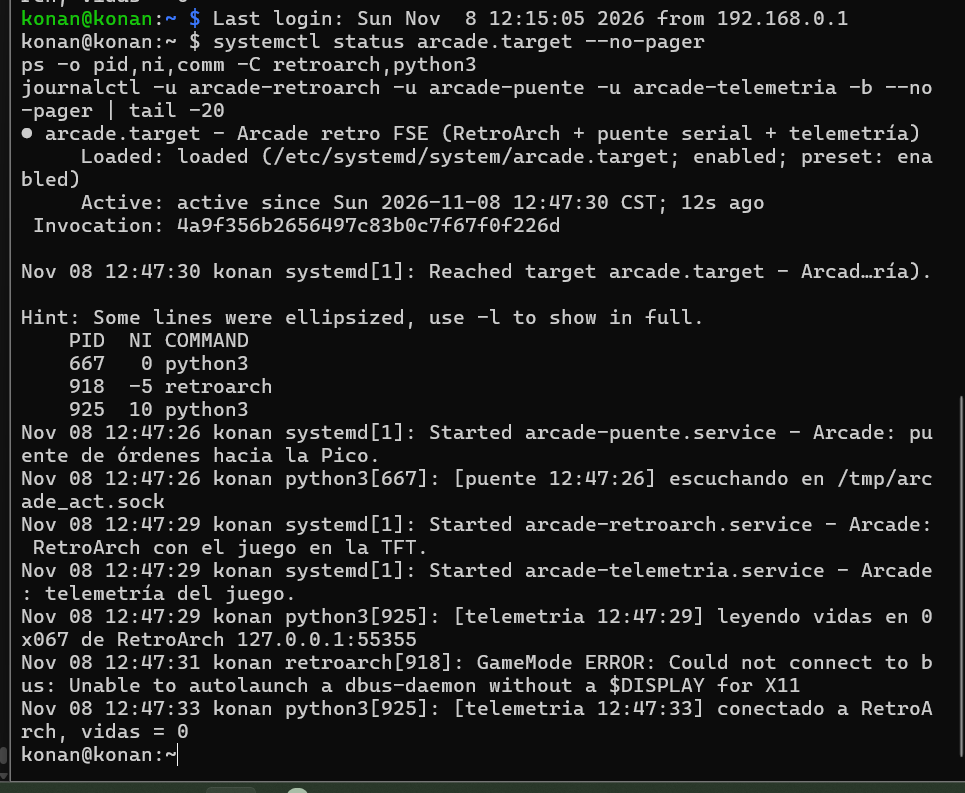
\includegraphics[width=0.85\columnwidth]{avance3/img/arranque_automatico.png}
	\caption{Prioridades de los procesos en la consola mostrando RetroArch con NI -5 y telemetría con NI 10.}
	\label{fig:nice}
\end{figure}

\textbf{Diferencias:} el \texttt{Nice} de la telemetría es 10 en lugar de 5 como se planeó originalmente, para asegurar que nunca interfiera con la emulación.

\subsection{Clase 9: Sincronización}
\textbf{Autor:} Hernández Alonso Antonio Adonahí

\textbf{Planeado:} mutex de hardware en la Pico para proteger la estructura compartida entre el Core 0 (USB) y la alarma que lee los botones; triple buffer con semáforos POSIX en la Pi para la comunicación entre procesos.

\textbf{Construido:}
\begin{itemize}
	\item \textbf{Pico:} no se requirió spin lock ni mutex. El DMA escribe cada campo de \texttt{g\_controls} con una sola transferencia de 16 bits y el USB copia campo por campo con lecturas atómicas de 16 bits (\texttt{controls\_snapshot} en \texttt{usb\_data\_tx.c}), garantizando que ningún valor se lea a medias.
	\item \textbf{Pi:} el puente es el único proceso que escribe en el dispositivo HID del control (\texttt{/dev/arcade\_hid}), eliminando carreras de escritura por diseño. El triple buffer lo implementa RetroArch mediante DRM (\texttt{ra\_gl.cfg}, línea 3261, \texttt{video\_max\_swapchain\_images = "3"}).
\end{itemize}

\textbf{Diferencias:} se planeó usar mutex de hardware en la Pico, pero el diseño final con transferencias atómicas de 16 bits eliminó la necesidad de sincronización explícita. Los semáforos POSIX planeados para el triple buffer no fueron necesarios porque RetroArch ya implementa su propio triple buffer a nivel de driver gráfico.
